\chapter{Implementační architektura a algoritmy hodnocení kvality}
\label{ch:grading}

Tato kapitola se zabývá rozhodovací logikou hodnotícího systému, který plně automatizuje proces třídění a vyřazování expozic. Architektura podsystému kombinuje exaktní fyzikální limity s relativními statistickými modely, což umožňuje pružně reagovat na proměnlivé podmínky během akvizičních nocí.

\section{Režimy vyhodnocování (Globální vs. relační analýza)}
Systém nabízí dva konfigurovatelné režimy pro relativní porovnávání snímků, které zásadně ovlivňují chování statistického modelu a výpočet distribucí:

\begin{enumerate}
    \item \textbf{Lokální režim (po skupinách):} Statistické distribuce a mezní hodnoty se konstruují nezávisle pro každou pozorování relaci (noc). Tento přístup je vysoce inertní vůči dlouhodobým změnám atmosférických podmínek a je ideální pro izolované zpracování dat, kde kvalita z jedné noci nesmí ovlivnit přísnost klasifikace noci druhé.
    \item \textbf{Globální režim (křížový):} Výpočet normálního rozdělení a směrodatných odchylek probíhá napříč celým importovaným datasetem bez ohledu na datum pořízení. Tento režim nachází uplatnění při dlouhodobých projektech (tzv. \textit{multi-night projekty}), kdy je žádoucí vyřadit všechny snímky podprůměrné kvality vzhledem k celkovému historickému standardu dané optické soustavy.
\end{enumerate}

\section{Dvouprůchodový matematický hodnotící model}
Vlastní analýza kvality probíhá sekvenčně ve dvou oddělených průchodech. V prvním průchodu se provádí extrakce absolutních geometrických a kontrastních charakteristik z každé obrazové matice (počet hvězd, index \ac{HFD}, excentricita a kontrast pozadí). Z těchto normalizovaných hodnot se pomocí lineární kombinace s pevně stanovenými penalizačními vahami vypočítává surové skóre kvality. Použité konstanty a matematické limity pro výpočet surového skóre jsou uvedeny v Tabulce~\ref{tab:constants}.

\begin{table}[htbp]
    \centering
    \small
    \begin{tabular}{lllc}
        \hline
        \textbf{Metrika} & \textbf{Váhová konstanta ($W$)} & \textbf{Saturační limit pro optimum} & \textbf{Maximální penalizace} \\ \hline
        Počet hvězd & $W_{\text{star}} = 1.0$ & $5000$ hvězd & $0$ hvězd \\
        Profil \ac{FWHM} & $W_{\text{fwhm}} = 1.0$ & $\le 1.5$ px & $\ge 6.0$ px \\
        Kontrast pozadí & $W_{\text{bg}} = 1.5$ & \textit{Minimální \ac{RMS}} & $\text{Kontrast} \ge 10.0$ \\
        Excentricita & $W_{\text{ecc}} = 0.6$ & $0.0$ (dokonalá kružnice) & $\ge 0.6$ \\
        Profil stopy (\textit{Trail}) & $W_{\text{trail}} = 2.0$ & Bez lineárních prvků & Detekován průtah \\ \hline
    \end{tabular}
    \caption{Přehled interních konstant, vah a matematických limitů.}
    \label{tab:constants}
\end{table}

Ve druhém průchodu dochází k transformaci surového bodování na relativní skóre v rozsahu $\langle 0.0, 1.0 \rangle$ pomocí konstrukce lokální nebo globální Gaussovy distribuční křivky. Pozice snímku v této statistické distribuci určuje jeho finální zařazení metodou tří směrodatných odchylek ($3\sigma$).

Kromě automatické kategorizace systém implementuje sekundární hodnotící vrstvu, která dává uživateli plnou kontrolu nad výslednou přísností selekce. Prostřednictvím konfiguračního rozhraní (viz Obrázek \ref{fig:thresholding}) lze dynamicky měnit spodní hranici akceptovatelnosti (\textit{rejection threshold}). Změna tohoto parametru okamžitě spustí znovu výpočet metrik a zajistí znovu klasifikaci snímků do správných kategorií na základě nové hranice akceptovatelnosti.

\begin{figure}[htbp]
    \centering
    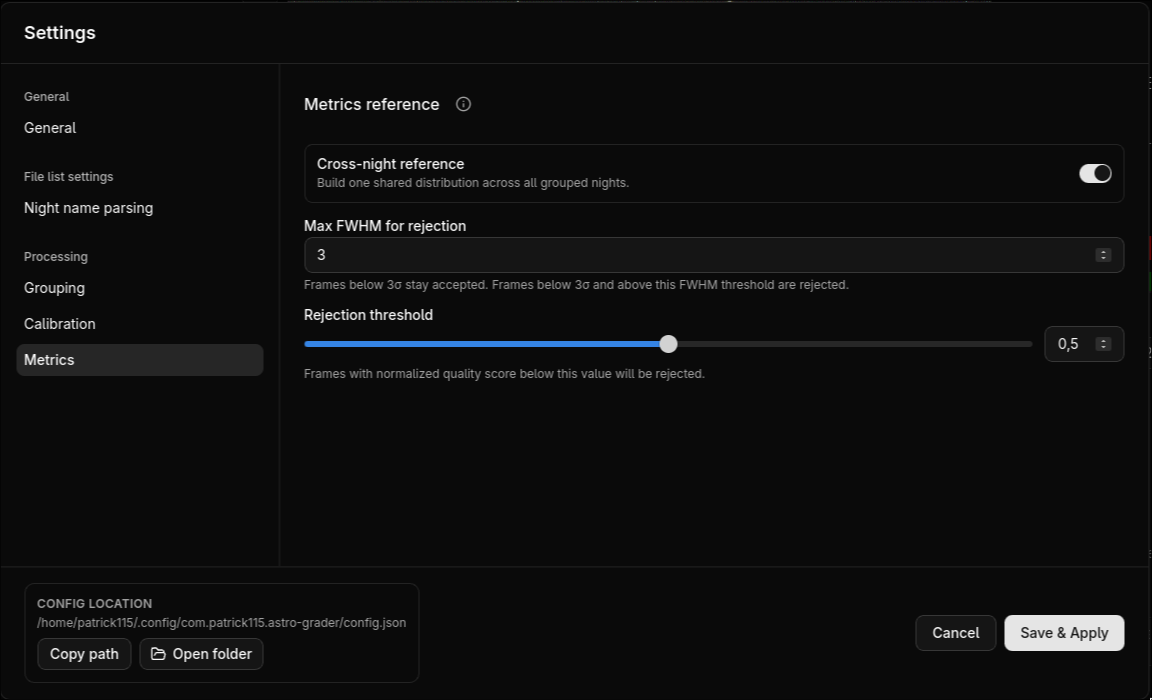
\includegraphics[width=0.60\textwidth]{assets/treshold_settings.png}
    \caption{Konfigurační panel uživatelského rozhraní pro dynamické nastavení prahových hodnot a spodní hranice akceptovatelnosti relativního skóre.}
    \label{fig:thresholding}
\end{figure}

\section{Ochranná logika a deterministické pojistky}
Aby se zabránilo selhání relativního statistického modelu v anomálních situacích (například pokud jsou vlivem souvislé oblačnosti znehodnoceny všechny snímky z dané noci, což by u čistě relativního modelu vedlo k chybnému schválení nejméně poškozených expozic), systém obsahuje autonomní ochranné pojistky.

Snímek je okamžitě klasifikován stavem vyřazení s příslušným chybovým hlášením bez ohledu na svou pozici v normálním rozdělení, pokud nastane jedno z následujících kritérií:
\begin{itemize}
    \item Celkový počet detekovaných bodových zdrojů klesne pod kritickou mez, což indikuje přítomnost husté oblačnosti nebo technické selhání expozice.
    \item Průměrná excentricita profilů hvězd překročí pevný práh $0.6$, což detekuje závažné mechanické chyby v pointaci montáže nebo přítomnost výrazných stop družic a meteorů (\textit{star trails}).
    \item Globální kontrast pozadí překročí absolutní kritickou hodnotu $15.0$ vlivem extrémního rozptylu světla na vysoké oblačnosti či při náhlém osvícení měsícem.
\end{itemize}

Všechny tyto metriky jsou zobrazeny v \ac{UI} a dovolují jednoduše uživateli vybrat zamítnuté (rejected) snímky a buď provést jejich smazání, nebo je přesunout do jiné složky (viz Obrázek \ref{fig:metrics_list}).

\begin{figure}[htbp]
    \centering
    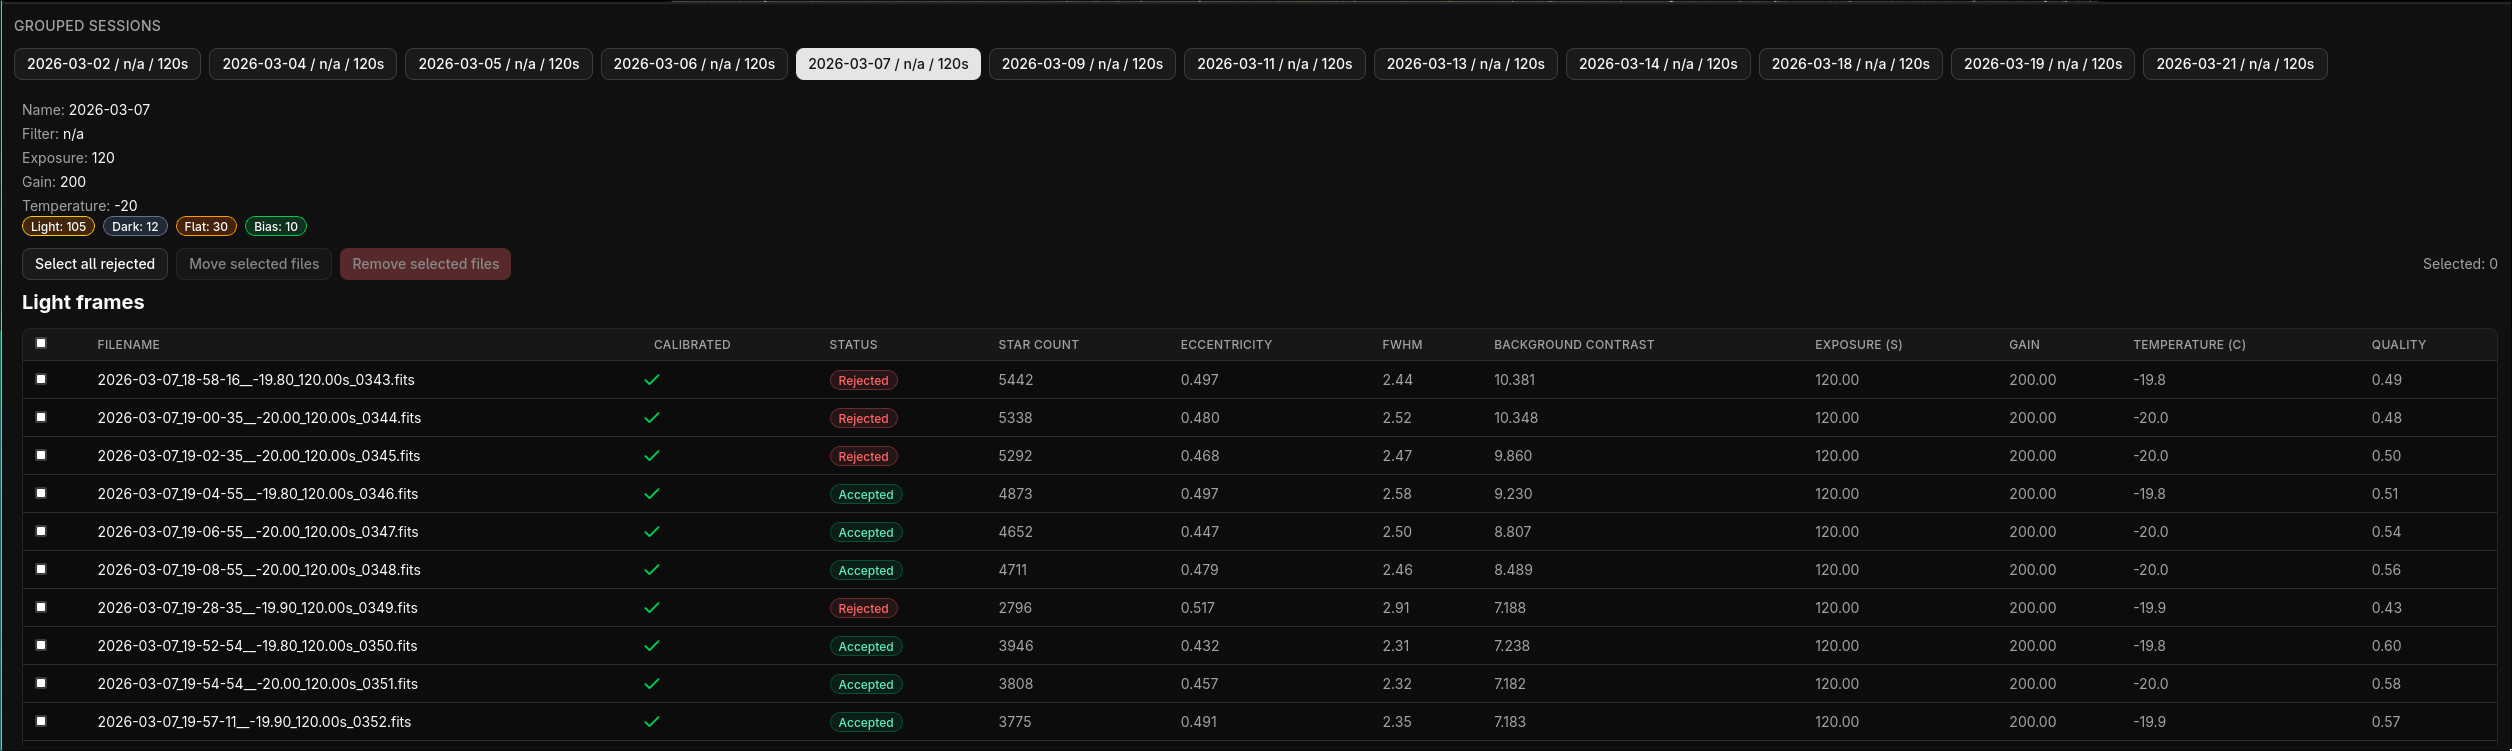
\includegraphics[width=0.85\textwidth]{assets/table.png}
    \caption{Ukázka vygenerovaného seznamu analyzovaných souborů v uživatelském rozhraní se zobrazením vypočtených fyzikálních metrik a finálního stavu.}
    \label{fig:metrics_list}
\end{figure}